\chapter*{ESSEC-I 2018 : le sujet}
  
%

\noindent
Dans tous le sujet :
\begin{noliste}{$\sbullet$}
\item on désigne par $n$ un entier naturel, au moins égal à $2$,
  
\item $X$ est une \var à valeurs dans un intervalle $]0,\alpha[$, où
  $\alpha$ est un réel strictement positif. On suppose que $X$ admet
  une densité $f$ strictement positive et continue sur $]0,\alpha[$,
  et nulle en dehors de $]0,\alpha[$.
  
\item on note $F$ la fonction de répartition de $X$.
  
\item $X_1$, $\ldots$, $X_n$ est une famille de \var mutuellement
  indépendantes et de même loi que $X$.
\end{noliste}
On admet que toutes les variables aléatoires considérées sont définies
sur le même espace probabilisé $(\Omega, \A, \Prob)$.


\section*{Partie I - Lois des deux plus grands}

\noindent
Les notations et résultats de cette partie seront utilisés dans le reste
du sujet.\\
On définit deux variables aléatoires $Y_n$ et $Z_n$ de la façon 
suivante.\\
Pour tout $\omega \in \Omega$ :
\begin{noliste}{$\sbullet$}
  \item $Y_n(\omega) = \max(X_1(\omega), \ldots, X_n(\omega))$ est le 
  plus grand des réels $X_1(\omega)$, $\ldots$, $X_n(\omega)$ ;\\
  on remarque que $Y_n$ est définie également lorsque $n$ vaut $1$, de 
  sorte que dans la suite du sujet on pourra considérer $Y_{n-1}$.
  
  \item $Z_n(\omega)$ est le \og deuxième plus grand \fg{} des nombres 
  $X_1(\omega)$, $\ldots$, $X_n(\omega)$, autrement dit, une fois que 
  ces $n$ réels sont ordonnés dans l'ordre croissant, $Z_n$ est 
  l'avant-dernière valeur. On note que lorsque la plus grande valeur 
  est présente plusieurs fois, $Z_n(\omega)$ et $Y_n(\omega)$ sont 
  égaux.
\end{noliste}

\begin{noliste}{1.}
  \setlength{\itemsep}{4mm}
  \item Loi de $Y_n$.\\
  Soit $G_n$ la fonction de répartition de $Y_n$.
  \begin{noliste}{a)}
    \setlength{\itemsep}{2mm}
    \item Montrer que pour tout réel $x$ : $G_n(x)=F(x)^n$.
    
    
    
    
    %\newpage

    
    \item En déduire que $Y_n$ est une variable aléatoire à densité 
    et exprimer une densité $g_n$ de $Y_n$ en fonction de $f$, $F$
    et $n$.
    
    

    
    \item Montrer que $Y_n$ admet une espérance.
    
    
  \end{noliste}
  
  
  %\newpage
  
  
  \item Loi de $Z_n$.\\
  Soit $H_n$ la fonction de répartition de $Z_n$.
  \begin{noliste}{a)}
    \setlength{\itemsep}{2mm}
    \item Soit $x$ un réel.
    \begin{nonoliste}{(i)}
      \item Soit $\omega \in \Omega$, justifier que $Z_n(\omega) \leq x$
      si et seulement si dans la liste de $n$ éléments $X_1(\omega)$,
      $\ldots$, $X_n(\omega)$, au moins $n-1$ sont inférieurs ou égaux
      à $x$.\\
      Donner une expression de l'événement $\Ev{Z_n \leq x}$ en 
      fonction des événements $\Ev{X_k \leq x}$ et $\Ev{X_k >x}$ avec
      $k \in \{1, \ldots, n \}$.
      
      
      
      
      %\newpage

      
      \item Établir : $H_n(x) = n(1-F(x))(F(x))^{n-1} + F(x)^n$.
      
      

    \end{nonoliste}
    
    \item Montrer que $Z_n$ est une variable à densité et qu'une 
    densité de $Z_n$ est donnée par :
    \[
      h_n(x) \ = \ n(n-1) \, f(x) \, (1-F(x))(F(x))^{n-2}
    \]
    
    
  \end{noliste}
  

  \newpage


  \item Simulation informatique.\\
  On suppose que l'on a défini une fonction \Scilab{} d'entête {\tt 
  function x = simulX(n)} qui retourne une simulation d'un échantillon 
  de taille $n$ de la loi de $X$ sous la forme d'un vecteur de 
  longueur $n$. Compléter la fonction qui suit pour qu'elle retourne le 
  couple $(Y_n(\omega), Z_n(\omega))$ associé à l'échantillon 
  simulé par l'instruction {\tt X = simulX(n)} :
  \begin{scilab}
     & \tcFun{function} [\tcVar{y}, \tcVar{z}] = 
     DeuxPlusGrands(\tcVar{n}) \nl %
     & \quad X = simulX(\tcVar{n}) \nl %
     & \quad \tcIf{if} ... \nl %
     & \quad \quad \tcVar{y} = X(1) ; \tcVar{z} = X(2) \nl %
     & \quad \tcIf{else} \nl %
     & \quad \quad ... \nl %
     & \quad \tcIf{end} \nl %
     & \quad \tcFor{for} k = 3:\tcVar{n} \nl %
     & \quad \quad \tcIf{if} X(k) > y \nl %
     & \quad \quad \quad \tcVar{z} = ... ; \tcVar{y} = ... \nl %
     & \quad \quad \tcIf{else} \nl %
     & \quad \quad \quad \tcIf{if} ... \nl %
     & \quad \quad \quad \quad \tcVar{z} = ... \nl %
     & \quad \quad \quad \tcIf{end} \nl %
     & \quad \quad \tcIf{end} \nl %
     & \quad \tcFor{end} \nl %
     & \tcFun{endfunction}
  \end{scilab}
  
  

  
  \item Premier exemple : loi uniforme.\\
  On suppose dans cette question que $X$ suit la loi uniforme sur 
  $]0,\alpha[$.
  \begin{noliste}{a)}
    \setlength{\itemsep}{2mm}
    \item Donner une densité de $Y_n$ et une densité de $Z_n$.
    
    

    
    \item Calculer l'espérance de $Y_n$ et de $Z_n$.
  \end{noliste}
\end{noliste}
    
    
  
  
  %\newpage
  
  \begin{noliste}{1.}
    \setcounter{enumi}{4}
    \setlength{\itemsep}{4mm}
  \item Deuxième exemple : loi puissance.\\
  On suppose dans cette question que la densité $f$ est donnée par :
  $f(x) = \left\{
  \begin{array}{cR{2cm}}
    \lambda \, \dfrac{x^{\lambda -1}}{\alpha^\lambda}
    & si $x \in \ ]0,\alpha[$ 
    \nl
    \nl[-.2cm]
    0 & sinon
  \end{array}
  \right.$
  où $\lambda$ est une constante strictement positive.\\
  On dit que $X$ suit la \emph{loi puissance} de paramètres 
  $\alpha$ et $\lambda$.
  \begin{noliste}{a)}
    \setlength{\itemsep}{2mm}
    \item 
    \begin{nonoliste}{(i)}
      \item Vérifier que $f$ est bien une densité de probabilité.
      
      
      
      
      %\newpage

      
      \item Déterminer la fonction de répartition $F$ de $X$.
      
      

      
      \item Calculer l'espérance de $X$.
      
      
    \end{nonoliste}
    
    
    %\newpage
    
    
    \item 
    \begin{nonoliste}{(i)}
      \item Montrer que $Y_n$ suit une loi puissance de paramètres 
      à préciser en fonction de $n$, $\lambda$ et $\alpha$.
      
      
      
      \item En déduire l'espérance de $Y_n$.
      
      
    \end{nonoliste}
    
    \item Calculer l'espérance de $Z_n$.
    
    
  \end{noliste}
\end{noliste}


\newpage

\section*{Partie II - Un problème d'optimisation}

\noindent
On reprend la notation de la partie précédente : $G_{n-1}$ est la
fonction de répartition de $Y_{n-1}$, qui est le maximum de $X_1$, 
$\ldots$, $X_{n-1}$.\\
On répond dans cette partie au problème d'optimisation suivant : 
trouver une fonction $\sigma$ définie sur $]0,\alpha[$ vérifiant les 
trois propriétés :
\begin{noliste}{$\sbullet$}
  \item $\sigma$ est une bijection de $]0,\alpha[$ dans un intervalle 
  $]0,\beta[$, avec $\beta$ un réel strictement positif.
  \item $\sigma$ est de classe $\Cont{1}$ sur $]0,\alpha[$ et 
  $\sigma'$ est à valeurs strictement positives sur $]0,\alpha[$.
  \item on définit, pour tout $x \in \ ]0,\alpha[$ et tout $y \in 
  \ ]0, \beta[$,
  \[
    \gamma(x,y) \ = \ (x-y) \, G_{n-1}(\sigma^{-1}(y))
  \]
  Alors pour tout $x \in \ ]0,\alpha[$, $\gamma(x,y)$ atteint son 
  maximum lorsque $y = \sigma(x)$.
\end{noliste}




\begin{noliste}{1.}
  \setlength{\itemsep}{4mm}
  \setcounter{enumi}{5}
  \item Analyse.\\
  On suppose dans un premier temps qu'une telle fonction $\sigma$ 
  vérifiant ces trois propriétés existe.
  \begin{noliste}{a)}
    \setlength{\itemsep}{2mm}
    \item Montrer que $\sigma^{-1}$ est dérivable sur $]0,\beta[$ et 
    exprimer sa dérivée $(\sigma^{-1})'$ en fonction de $\sigma'$
    et $\sigma^{-1}$.
    
    
    
    
    %\newpage

    
    \item Calculer la dérivée partielle $\dfn{\gamma}{2}(x, y)$.
    
    

    \item Montrer que pour tout $x \in \ ]0, \alpha[$, on a 
    $\dfn{\gamma}{2}(x, \sigma(x))=0$.\\
    En déduire que pour tout $x \in \ ]0, \alpha[$ : 
    \[
      \sigma'(x) \, G_{n-1}(x) + \sigma(x) \, g_{n-1}(x) \ = \
      x \, g_{n-1}(x)
    \]
    
    

    
    \item Montrer alors, pour tout $x \in \ ]0,\alpha[$ : 
    \[
      \sigma(x) \ = \ \dfrac{1}{G_{n-1}(x)} \, \dint{0}{x} t \, 
      g_{n-1}(t) \dt \qquad (*)
    \]
    
    
    
    \item À l'aide d'une intégration par parties, montrer que pour tout
    $x \in \ ]0,\alpha[$, on a également : 
    \[
      \sigma(x) \ = \ x - \dint{0}{x} \dfrac{G_{n-1}(t)}{G_{n-1}(x)}
      \dt \qquad (**)
    \]
    
    
  \end{noliste}
  
  \item Synthèse.\\
  On suppose à présent que $\sigma$ est la fonction définie par 
  l'égalité $(*)$ ou $(**)$.
  \begin{noliste}{a)}
    \setlength{\itemsep}{2mm}
    \item Montrer que pour tout $x \in \ ]0, \alpha[$, $0 < \sigma(x)
    <x$.
    
    

    
    \item Montrer que $\sigma$ est de classe $\Cont{1}$ sur $]0,\alpha[$
    et que pour tout $x \in \ ]0,\alpha[$, $\sigma'(x)$ est du signe 
    de $x- \sigma(x)$.\\
    En déduire que $\sigma'$ est strictement positive sur $]0,\alpha[$.
    
    
    
    \item Montrer que $\sigma$ réalise une bijection de $]0,\alpha[$
    dans $]0,\beta[$, avec $\beta = \E(Y_{n-1})$.
    
    
    
    
    %\newpage

    
    \item On fixe un réel $x \in \ ]0, \alpha[$. Soit $y \in \ ]0, 
    \beta[$, on pose $z= \sigma^{-1}(y)$.
    \begin{nonoliste}{(i)}
      \item Établir : 
      \[
        \gamma(x,y) \ = \ (x-z) \, G_{n-1}(z) + \dint{0}{z} G_{n-1}(t)
        \dt
      \]
      
      
      
      \item En déduire : $\gamma(x, \sigma(x)) - \gamma(x,y) \ = \
      (z-x) \, G_{n-1}(z) - \dint{x}{z} G_{n-1}(t) \dt$.
      
      
      
      
      %\newpage

      
      \item Déterminer le signe de $\gamma(x, \sigma(x)) - 
      \gamma(x,y)$ et conclure que $\gamma(x,y)$ est maximal lorsque\\ 
      $y = \sigma(x)$.
      
      
    \end{nonoliste}
  \end{noliste}
  

  \newpage


  \item Estimation de $\sigma(x)$.\\
  Soit $x \in \ ]0,\alpha[$.
  \begin{noliste}{a)}
    \setlength{\itemsep}{2mm}
    \item On considère la fonction $\varphi_x$ définie sur $\R_+$ par :
    $\varphi_x(t) = 
    \left\{
    \begin{array}{cR{2cm}}
      t & si $t \leq x$
      \nl
      0 & sinon
    \end{array}
    \right.$\\[.2cm]
    En utilisant la relation $(*)$, montrer que $\sigma(x) = 
    \dfrac{\E(\varphi_x(Y_{n-1}))}{\Prob(\Ev{Y_{n-1} \leq x})}$.
    
    
    
    
    %\newpage

    
    \item En déduire une fonction \Scilab{} {\tt function s = 
    sigma(x,n)} qui retourne une valeur approchée de $\sigma(x)$
    obtenue comme quotient d'une estimation de $\E(\varphi_x(Y_{n-1}))$
    et de $\Prob(\Ev{Y_{n-1} \leq x})$.\\
    On utilisera la fonction {\tt simulX} pour simuler des 
    échantillons de la loi de $X$, et on rappelle que si {\tt v} est 
    un vecteur, {\tt max(v)} est égal au plus grand élément de 
    {\tt v}.
    
    
  \end{noliste}
  
  
  %\newpage
  
  
  \item Exemples.\\
  Donner une expression de $\sigma(x)$ pour tout $x \in \ ]0,\alpha[$
  dans les cas suivants : 
  \begin{noliste}{a)}
    \setlength{\itemsep}{2mm}
    \item $X$ suit la loi uniforme sur $]0,\alpha[$.
    
    

    
    \item $X$ suit la loi puissance de paramètres $\alpha$ et $\lambda$.
    Votre résultat est-il en accord avec la courbe ci-dessous 
    obtenue sous cette hypothèse, en utilisant la fonction {\tt sigma}
    de la question précédente lorsque $n=6$, $\lambda=0,2$ et 
    $\alpha = 50$ ? Justifier votre réponse.
    
    \begin{center}
      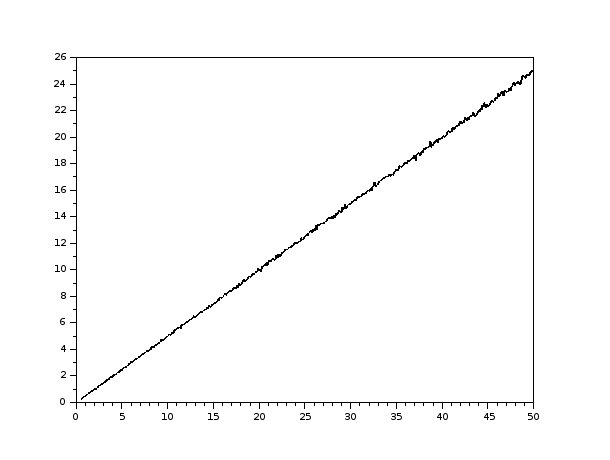
\includegraphics[scale=.5]
      {Figures/ESSEC-I_2018/Figure_ESSEC-I_2018.png}
    \end{center}
    
    
    %\newpage
    
    
    
  \end{noliste}
\end{noliste}



\newpage



\section*{Partie III - Modélisation d'enchères}

\noindent
Un bien est mis en vente aux enchères et $n$ acheteurs $A_1$, $\ldots$,
$A_n$ sont intéressés. Chaque acheteur $A_k$ attribue une valeur $x_k$ 
à ce bien, appelée \emph{valeur privée}, qui n'est pas connue des 
autres acheteurs. Afin de se procurer ce bien, $A_k$ propose ensuite, 
de façon secrète, une \emph{mise} (on dit aussi une \emph{offre}) 
$y_k$. Toutes les mises sont alors révélées simultanément et l'acheteur 
qui remporte le bien est celui qui a proposé la plus grande mise. En 
cas d'égalité, le gagnant est tiré au sort parmi ceux qui ont la mise 
la plus importante.\\
Le prix à payer par le gagnant au vendeur dépend du type d'enchère 
organisé. On étudie ici deux formats d'enchères :
\begin{noliste}{$\sbullet$}
  \item l'\emph{enchère au premier prix}, ou enchère hollandaise : 
  l'acheteur gagnant paye la mise qu'il a lui-même proposée. Ce type 
  d'enchère correspond aux enchères dynamiques \og descendantes \fg{} :
  la vente commence avec un prix très élevé et baisse progressivement.
  Le premier qui accepte le prix remporte le bien.
  
  \item l'\emph{enchère au second prix}, ou enchère anglaise : 
  l'acheteur gagnant paye le prix correspondant à la deuxième meilleure
  mise.\\
  Ce type d'enchère est presque équivalent aux enchères dynamiques \og
  montantes \fg{} bien connues : le prix monte progressivement 
  jusqu'à ce qu'il ne reste plus qu'un seul acheteur : celui qui est 
  prêt à mettre le plus haut prix, et qui paye (à peu de chose près) le
  prix de la deuxième offre après la sienne.
\end{noliste}
Pour chaque acheteur $A_k$, on appelle \emph{résultat net} ou 
simplement \emph{résultat} de l'enchère, et on note $r_k$, le bénéfice 
ou le perte résultant de l'opération. Pour l'acheteur qui a remporté 
l'enchère, le résultat est la différence entre la valeur privée et le 
prix payé. Pour les autres acheteurs, le résultat est considéré comme 
nul.\\
À titre d'exemple, considérons quatre acheteurs, dont les mises en 
euros sont $y_1=50$, $y_2=100$, $y_3=80$ et $y_4=40$, alors l'acheteur 
$A_2$ gagne l'enchère. Si sa valeur privée $x_2$ vaut $90$ euros, il 
paye $100$ euros au vendeur pour un résultat de $r_2=-10$ euros s'il 
s'agit d'une enchère au premier prix, et $80$ euros pour un résultat de 
$r_2=10$ euros si c'est une enchère au second prix.\\
On s'intéresse au problème suivant : à partir de l'information dont 
dispose l'acheteur $k$, notamment à partir de sa valeur privée $x_k$, 
comment doit-il choisir sa mise $y_k$ afin d'optimiser son résultat net 
? On appelle \emph{stratégie} de l'acheteur $k$ une fonction $\sigma_k$ 
telle que $y_k = \sigma_k(x_k)$.



\subsection*{1- Enchère au premier prix}

\noindent
On suppose que chaque acheteur $A_k$ a une valeur privée $x_k = 
X_k(\omega)$ qui est une réalisation de la variable aléatoire $X_k$.\\
Soit $\sigma$ la fonction définie à la partie II.\\
Le problème étant symétrique, on se met par exemple à la place de 
l'acheteur $n$, et on suppose que les $n-1$ premiers acheteurs 
appliquent la stratégie $\sigma$, c'est-à-dire : pour tout $k\in \{1, 
\ldots, n-1\}$, l'acheteur $k$ mise $\sigma(X_k)$.\\
L'acheteur $n$ a une valeur privée $x_n$ et choisit une mise $y_n$.\\
On note $E_n$ l'événement \og l'acheteur $A_n$ remporte l'enchère \fg{}.
\begin{noliste}{1.}
  \setlength{\itemsep}{4mm}
  \setcounter{enumi}{9}
  \item En remarquant que $\Prob(\Ev{Y_{n-1} = \sigma^{-1}(y_n)}) = 0$,
  montrer que $\Prob(E_n) = \Prob(\Ev{Y_{n-1} < \sigma^{-1}(y_n)})$.\\
  On note $R_n$ la variable aléatoire donnant le résultat net de 
  l'enchère pour l'acheteur $A_n$.\\
  Justifier que $R_n = (x_n-y_n) \, \unq{}_{E_n}$ et en déduire que le 
  résultat espéré de l'acheteur $A_n$ en fonction de sa valeur 
  privée $x_n \in \ ]0,\alpha[$ et de l'offre $y_n \in \ ]0,\beta[$ 
  est donné par :
  \[
    \E(R_n) \ = \ (x_n-y_n) \, G_{n-1}(\sigma^{-1}(y_n))
  \]
  
  
  %\newpage
  
  
  
  
  \item En déduire que pour optimiser son espérance de résultat, 
  l'acheteur $A_n$ a intérêt à appliquer lui aussi la stratégie 
  $\sigma$.\\
  Il s'agit de ce que l'on appelle un \emph{équilibre de Nash} en 
  théorie des jeux : si tous les acheteurs appliquent cette 
  stratégie d'équilibre $\sigma$, alors aucun n'a intérêt à 
  changer de stratégie.
  
  
\end{noliste}



%\newpage



\subsection*{2- Enchère au second prix}

\noindent
On se met à nouveau à la place de l'acheteur $n$. Soit $m = \max(y_1, 
\ldots, y_{n-1})$ la meilleure offre faite par les acheteurs $A_1$, 
$\ldots$, $A_{n-1}$ (que $A_n$ ne connaît pas).
\begin{noliste}{1.}
  \setlength{\itemsep}{4mm}
  \setcounter{enumi}{11}
  \item \begin{noliste}{a)}
    \setlength{\itemsep}{2mm}
    \item Si on suppose que $m \geq x_n$, montrer que quelle que soit la
    mise $y_n$, le résultat net $r_n$ pour $A_n$ est négatif ou nul. 
    Que vaut $r_n$ pour le choix $y_n = x_n$ ?
    
    

    
    \item Si on suppose que $m < x_n$, quel est le résultat pour $A_n$
    dans les cas $y_n < m$ et $y_n \geq m$ ?
    
    

    
    %\newpage
    
    
    \item En déduire que la meilleure stratégie pour $A_n$ consiste 
    à prendre $y_n =x_n$.
    
    
  \end{noliste}
\end{noliste}
Par symétrie, chaque acheteur a également intérêt à miser le montant de 
sa valeur privée. On parle de \emph{stratégie dominante} : chaque 
acheteur a une stratégie optimale indépendamment du comportement des 
autres acheteurs.




\subsection*{3- Équivalence des revenus}


\noindent
On se met maintenant à la place du vendeur.\\
Les valeurs privées des acheteurs sont données par les variables 
aléatoires $X_1$, $\ldots$, $X_n$.
\begin{noliste}{1.}
  \setlength{\itemsep}{4mm}
  \setcounter{enumi}{12}
  \item Enchère au premier prix.\\
  On suppose que le vendeur organise une enchère au premier prix, et 
  que les acheteurs adoptent la stratégie d'équilibre $\sigma$ donnée
  à la partie III-1.\\
  On note $B_n$ la variable aléatoire donnant le \emph{bénéfice}, ou 
  \emph{revenu}, du vendeur. Il s'agit du montant que paye l'acheteur
  qui a remporté l'enchère.
  \begin{noliste}{a)}
    \setlength{\itemsep}{2mm}
    \item Justifier que $B_n = \sigma(Y_n)$.
    
    
    
    
    %\newpage

    
    \item En déduire :
    \[
      \E(B_n) \ = \ n \, \dint{0}{\alpha} \sigma(x) \, G_{n-1}(x) \,
      f(x) \dx \ = \ n \, \dint{0}{\alpha} \left( \dint{0}{x} t \, 
      g_{n-1}(t) \dt \right) f(x) \dx
    \]
    
    

    
    \item Montrer, à l'aide d'une intégration par parties :
    \[
      \E(B_n) \ = \ n \, \dint{0}{\alpha} x \, (1-F(x)) \, 
      g_{n-1}(x) \dx
    \]
    
    
  \end{noliste}
  
  \item Enchère au second prix.\\
  On suppose que le vendeur organise une enchère au second prix, et que 
  les acheteurs adoptent la stratégie dominante de la partie III-2 : 
  chacun mise autant que sa valeur privée.\\
  On note $B_n'$ la variable aléatoire donnant le revenu du vendeur 
  dans cette enchère.\\
  Justifier que $\E(B_n') = \E(Z_n)$.
  
  

  
  \item Établir : $\E(B_n) = \E(B_n')$.
  
  
\end{noliste}
Ainsi, le revenu moyen pour le vendeur est le même pour les enchères au 
premier ou au second prix lorsque les acheteurs adoptent tous la 
stratégie optimale. Plus généralement, on peut montrer que ce revenu 
moyen est encore le même dans une très grande classe de formats 
d'enchères, ce résultat portant le nom de \emph{principe d'équivalence 
du revenu}.






